\section{Casos que harían que el proyecto dejará de funcionar}

\subsection{Servicio del back-end no activo}
Evidentemente si el servidor no está activo y con la capacidad para recibir peticiones el programa no podrá funcionar y tendrá una salida parecida a la siguiente.

\begin{center}
	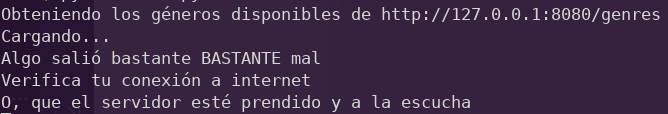
\includegraphics[width=0.75\linewidth]{error-server}
	\captionof{figure}{Salida de la aplicación cuando el backend no está activo}
\end{center}

\subsection{Otros casos menores}
Fuera de los casos donde deja de funcionar la aplicación, existen casos en los que la aplicación no funciona correctamente pero sigue funcionando, tales son los casos en los que la visualización por página se desacomoda momentaneamente al hacer scroll, o que no se muestren los detalles completos de una película o episodio si su nombre es bastante largo. De igual forma existe un pequeño bug en la visualización de los resultados por paginación si el número de resultados no es múltiplo de 5, al colocarse en la última página, supongamos que por no ser múltiplo de 5 la cantidad de resultados que se muestran son simplemente 3 y después se regresa a la primera página en la cual aparecerán en vez de 5 resultados, 3 resultados. Este es un error de visualización, sin embargo no representa ninguna pérdida de datos y todos los resultados se pueden seguir viendo, para solucionar dicho problema se tendría que modificar el incremento o decremento de una variable que controla la paginación en la clase PaginationControls.

Por otro lado, normalmente no se podrá ejecutar la aplicación si tanto para el backend como para el frontend (la aplicación de python) no se tienen instaladas las dependencias requeridas, por lo que será necesario instalarlas simplemente con \mono{pip install -r <ruta hacia el archivo requirements.txt>}, dicho archivo \mono{requirements.txt} contiene las dependencias y versiones requeridas para ejecutar el frontend.

Asimismo, naturalmente pueden existir fallas en la aplicación debidas no al código de la aplicación directamente, sino al código externo utilizado adentro de este mismo proyecto, por ejemplo, en la clase Request donde se utiliza un queue, es posible que existan fallos a pesar de que se programó de forma que se eviten tales inconvenientes, pero, de la misma documentación de Python se conoce que los métodos no pueden funcionar como uno espera, e. g. "$\:$If empty() returns True it doesn’t guarantee that a subsequent call to put() will not block. Similarly, if empty() returns False it doesn’t guarantee that a subsequent call to get() will not block.", obtenido de la documentación de python  (ver referencias), y lo mismo aplica para el backend.